% ============================================================
% CHAPITRE 3 : ÉTUDE DE FAISABILITÉ
% ============================================================

\setcounter{chapter}{2}
\chapter{Étude de la faisabilité}

L'étude de faisabilité consiste à évaluer la faisabilité d'un projet avant sa mise en œuvre. Elle vise à déterminer si le projet est réalisable sur le plan technique, le plan économique, le plan juridique et le plan organisationnel : sur le plan technique, il s'agit de vérifier s'il est possible de réaliser le projet et quelles ressources matérielles, humaines et technologiques sont nécessaires ; sur le plan de la rentabilité économique, d'évaluer la viabilité financière du projet, les coûts prévus, les bénéfices attendus et la rentabilité escomptée ; sur le plan juridique, de vérifier le respect des lois et règlementations en vigueur ainsi que les contraintes légales ou autorisations spécifiques à obtenir ; et sur le plan organisationnel, d'examiner si le projet peut être mis en place dans l'organisation existante et quels changements organisationnels seraient nécessaires. Dans ce chapitre, nous nous attarderons tout d'abord sur l'étude de la faisabilité technique, dans la suite nous présenterons la structure organisationnelle de notre entreprise, et nous finirons par l'étude de la faisabilité fiscale et juridique.

\section{Étude de la faisabilité technique}

L'étude de la faisabilité d'un projet consiste à évaluer la faisabilité technique de la mise en œuvre d'un projet. Elle permet de déterminer si les ressources techniques nécessaires sont disponibles et si elles peuvent être mises en place pour réaliser le projet. Cette étude comprend l'analyse des différentes solutions techniques possibles, la définition des exigences techniques, l'identification des contraintes, risques et des obstacles potentiels techniques associés au projet.

Les différents paramètres légaux, environnementaux et techniques pour le déploiement de notre solution constituent des éléments déterminants. De l'utilisation des différentes technologies, jusqu'aux recherches dans les centres spécialisés, chaque aspect technique a été minutieusement étudié pour garantir la robustesse et la fiabilité d'Argos.

L'étude de la faisabilité technique est essentielle pour garantir que le projet peut être mis en œuvre avec succès et dans les délais impartis.

Sur le plan technique, plusieurs points critiques sont susceptibles de bloquer le projet Argos s'ils ne sont pas anticipés dès la conception. Cinq risques majeurs ont été identifiés, chacun assorti d'une solution technique retenue :

\begin{itemize}
    \item \textbf{Énergie et autonomie :} un trajet maritime Douala--Chine dure environ 45 jours ; si le boîtier tombe en panne d'énergie avant ce délai, aucune donnée n'est disponible sur le reste du trajet. La solution retenue associe une batterie de capacité SOC 12 à un mode « deep sleep », permettant de couvrir jusqu'à 90 jours d'autonomie.
    \item \textbf{Connectivité en haute mer :} près de 70~\% du trajet s'effectue en zone blanche, sans couverture 4G ni Wi-Fi, rendant impossible l'envoi immédiat d'une alerte (par exemple « conteneur ouvert »). La solution combine un stockage local des données avec un envoi en rafale dès l'arrivée au port, complété par une option de communication satellite Iridium pour les alertes critiques ; cette option satellite reste toutefois environ cinq fois plus coûteuse que les autres moyens de transmission.
    \item \textbf{Vol ou destruction du dispositif :} le boîtier peut être arraché ou détérioré par des voleurs ou lors des opérations de manutention portuaire. La solution consiste à utiliser un scellement de type « bolt seal », qui déclenche une alerte en cas d'arrachement.
    \item \textbf{Cybersécurité :} le dispositif est exposé à un risque de piratage visant à falsifier les données collectées. La solution retenue repose sur un chiffrement AES-256 associé à un horodatage des journaux (logs), potentiellement renforcé par une architecture de type blockchain\cite{loi2010_cyber}.
    \item \textbf{Interférences GPS :} un brouillage peut fausser la position rapportée, rendant impossible la preuve du lieu réel d'un vol. La solution combine une antenne GPS multi-constellation et une triangulation LoRa pour fiabiliser la géolocalisation.
\end{itemize}

En conclusion, tous ces points critiques sur le plan technique disposent de solutions identifiées, ce qui confirme la faisabilité technique du projet Argos. Cette analyse est développée plus en détail dans la sous-partie intitulée « Analyse » du chapitre 5 portant sur l'étude technique.


\section{Structure organisationnelle de l'entreprise}

La structure organisationnelle tire son origine de la théorie des organisations. Dans le cas d'une entreprise, elle définit le cadre hiérarchique et fonctionnel de l'entreprise organisant la répartition des tâches, des responsabilités et relations internes afin d'atteindre les différents objectifs. Concrètement, elle permet de préciser les quatre points essentiels qui sont :

\begin{itemize}
    \item Quels sont les différents services de l'organisation ?
    \item Quelles sont les responsabilités de chacun ?
    \item Comment les acteurs collaborent entre eux ?
    \item Comment s'exercent l'autorité et la circulation de l'information ?
\end{itemize}

La structure organisationnelle d'une entreprise permet donc de définir clairement les différents services, les responsabilités de chacun et les relations entre les acteurs. Elle facilite la répartition des tâches, améliore la coordination entre les employés et assure une bonne circulation de l'information à travers les niveaux hiérarchiques. Grâce à elle, chaque membre sait ce qu'il doit faire et à qui il doit rendre compte, ce qui rend le travail plus efficace et mieux organisé. Ainsi, elle joue un rôle essentiel dans le bon fonctionnement, la performance et l'atteinte des objectifs de l'entreprise.

La structure organisationnelle d'une entreprise comprend une représentation graphique dans sa structure appelée organigramme. Permettant de visualiser de manière synthétique la hiérarchie, les relations fonctionnelles ainsi que la répartition des responsabilités entre les différents services et acteurs de l'organisation.

Il nous revient, de présenter l'organigramme de l'entreprise d'abord, ensuite la répartition des responsabilités et des missions fonctionnelles.

\subsection{Organigramme de l'entreprise}

L'organigramme vise à visualiser l'agencement interne de l'entreprise, en mettant donc en évidence la distribution des responsabilités, les relations de subordination ainsi que les interactions entre les différentes entités organisationnelles. L'organigramme présente un intérêt stratégique pour plusieurs catégories d'acteurs :

\begin{itemize}
    \item \textbf{Le personnel :} l'organigramme d'une entreprise permet à chaque personnel de connaître sa position dans l'entreprise, de comprendre ses responsabilités, de savoir à qui rendre compte, et de faciliter la collaboration avec les autres services.
    \item \textbf{La direction générale :} l'organigramme d'une entreprise, vu sous l'angle de la direction générale, lui permet d'avoir une vue globale de l'organisation, de mieux répartir les tâches et responsabilités, de contrôler et coordonner les activités, et afin de faciliter la prise de décisions stratégiques.
    \item \textbf{Les clients de l'entreprise :} l'organigramme permet aux clients d'identifier les différents services de l'entreprise, de savoir à qui s'adresser selon leurs besoins, de mieux comprendre le fonctionnement de l'entreprise.
\end{itemize}

\begin{figure}[htbp]
    \centering
    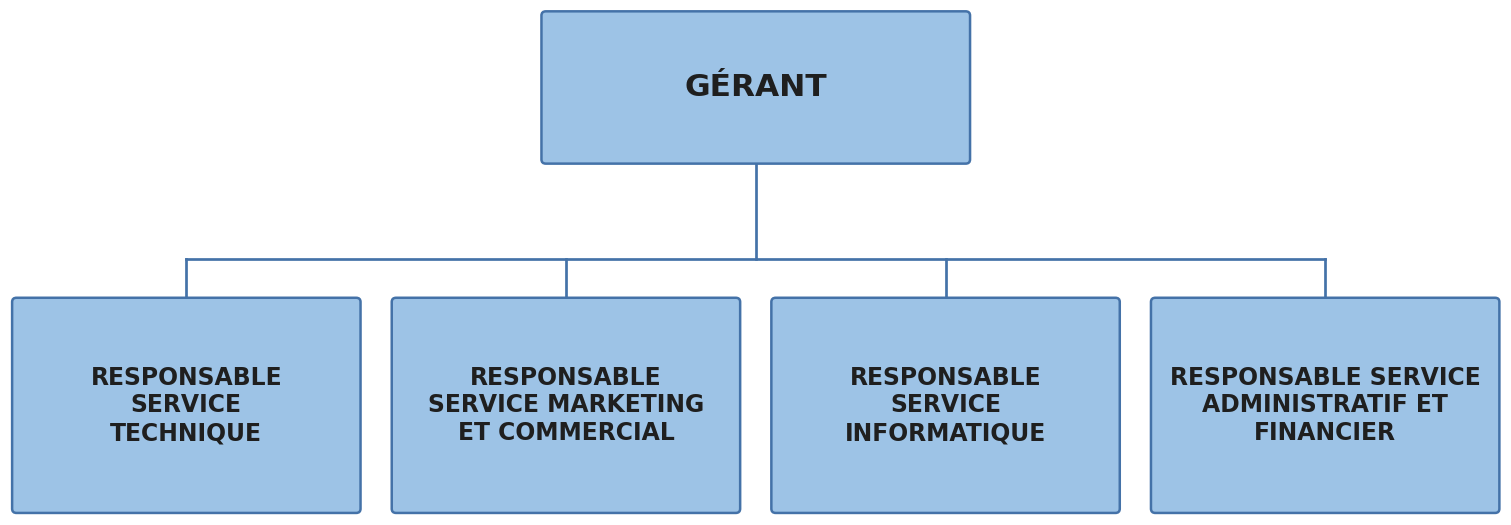
\includegraphics[width=0.9\textwidth]{capt1.png}
    \caption{Organigramme prévisionnel de l'entreprise}
    \label{fig:organigramme}
  \tablesourcepromoteurs

\end{figure}

\subsection{Définition des fonctions et attributions}

Dans toute organisation, chaque poste occupe une place précise et joue un rôle décisif dans le bon fonctionnement de l'ensemble. Les fonctions et attributions permettent de définir clairement les missions confiées à chaque responsable, afin d'assurer une meilleure répartition du travail, une bonne coordination des activités et une meilleure efficacité. La définition des fonctions vise à préciser les tâches, les responsabilités et les domaines d'intervention de chaque acteur de l'entreprise. Les attributions, quant à elles, déterminent les pouvoirs et les actions que chaque responsable est habilité à exercer dans le cadre de ses missions. Cette action d'organisation permet d'éviter les conflits de compétence, de faciliter la communication interne et de garantir l'atteinte des objectifs fixés par l'entreprise. Dans le cadre de ce projet, l'entreprise s'articule autour des postes suivants :
\begin{itemize}
        
    \item \textbf{Le Gérant}
    Il coiffe l'ensemble des autres services de l'entreprise; occupe une place centrale dans la structure organisationnelle et assure la coordination globale des activités en dirigeant, coordonnant, contrôlant et orientant toutes les activités vers la réalisation des objectifs fixés. Veille au fonctionnement intégral de chaque service en s'assurant que toutes les tâches sont correctement exécutées et en conformité avec les objectifs fixés par l'organisation. Le Gérant coordonne, organise et supervise les différentes actions menées au sein de l'entreprise afin d'assurer une bonne cohérence entre les services. En effet, il analyse les résultats obtenus, corrige les éventuels dysfonctionnements et met en place des stratégies pour améliorer la performance globale de l'entreprise. De plus, il sert de lien entre les différents services, favorisant ainsi une meilleure communication interne et une meilleure coordination du travail.

    \item \textbf{Responsable Service Technique}
    Le responsable du service technique constitue le cœur opérationnel du projet. Il est chargé de superviser et de coordonner l'ensemble des activités techniques de l'entreprise. Il veille au bon fonctionnement des équipements et des installations, organise les interventions de maintenance et s'assure de la qualité des travaux réalisés. Il garantit également le respect des normes de sécurité et propose des solutions techniques pour améliorer la performance et l'efficacité des services.

    \item \textbf{Responsable Service Marketing et Commercial}
    Le responsable du service marketing et commercial est un professionnel chargé à la fois de l'analyse du marché, de la définition des stratégies marketing et du développement des ventes de l'entreprise. Il étudie les besoins des consommateurs et la concurrence afin de proposer des actions adaptées pour promouvoir les produits ou services.
    Il met en place des campagnes de communication et des stratégies commerciales visant à attirer de nouveaux clients et à fidéliser la clientèle existante. Il participe également à la fixation des objectifs de vente, à la négociation avec les clients et au suivi des performances commerciales.
    En outre, il veille à la bonne image de l'entreprise, à la satisfaction des clients et à l'amélioration continue du chiffre d'affaires. Ainsi, il occupe un rôle essentiel dans la croissance et la compétitivité de l'organisation.

    \item \textbf{Responsable Service Informatique}
    Le responsable du service informatique est chargé du développement, du déploiement et de la maintenance de la plateforme logicielle d'Argos (application web d'administration, application mobile, API). Il s'occupe de l'administration des systèmes, des bases de données et de l'infrastructure cloud, ainsi que de la sécurité informatique et de la protection des données collectées. Il veille également à l'intégration des dispositifs embarqués avec la plateforme, au bon fonctionnement des serveurs et au support technique informatique auprès des autres services.

    \item \textbf{Responsable Service Administratif et Financier}
    Le responsable du service administratif et financier est chargé de la gestion des ressources financières de l'entreprise. Il veille à la bonne utilisation des fonds, à l'équilibre des dépenses et des recettes, ainsi qu'à la rentabilité des activités. Il élabore et suit le budget, contrôle les opérations comptables et financières, et s'assure du respect des obligations financières et fiscales. Il analyse également la situation financière de l'entreprise afin de proposer des solutions pour optimiser la gestion et soutenir la prise de décision. Sur le plan administratif, il assure également la gestion du personnel et des dossiers administratifs, le suivi des contrats et le respect des obligations légales et réglementaires de l'entreprise.


\end{itemize}
\subsection{Étude des ressources humaines}

Les ressources humaines jouent un rôle important dans le fonctionnement et la performance d'une entreprise. Elles permettent de valoriser le capital humain en assurant une bonne gestion du personnel, depuis le recrutement jusqu'à l'exploitation optimale des compétences de ce dernier. Elles contribuent à affecter les bonnes personnes aux bons postes, ce qui améliore l'efficacité et la productivité de l'organisation.

\subsubsection{Analyse des profils de poste}

Dans le but d'appréhender efficacement la répartition des rôles au sein de l'entreprise, il est nécessaire de procéder à une analyse des profils de poste. Cette démarche met en évidence les exigences propres à chaque fonction, tant en termes de compétences que de responsabilités.


\begin{table}[htbp]
    \centering
    \caption{Compétences relatives à chaque poste de responsabilité}
    \label{tab:competences}
    \renewcommand{\arraystretch}{1.5}
    \begin{tabularx}{\textwidth}{|>{\raggedright\arraybackslash}p{3cm}|X|X|}
        \hline
        \textbf{Postes de responsabilité} & \textbf{Buts recherchés} & \textbf{Compétences clés attendues} \\
        \hline
        \textbf{Gérant} & Veille au bon fonctionnement de chaque service de l'entreprise; oriente toutes les activités vers l'atteinte des objectifs de l'entreprise; s'assure de l'exécution correcte des tâches selon chaque service. & Sens du leadership, une vision globale et stratégique; capacité de prise de décision stratégique rapide et efficace; esprit d'analyse et de synthèse. \\
        \hline
        \textbf{Responsable Service Technique} & Organiser et coordonner les équipes techniques; assurer le bon fonctionnement des équipements et des installations (veiller à la maintenance préventive et corrective du matériel); contrôler la qualité des travaux techniques réalisés et s'assurer du respect des normes de sécurité et des procédures techniques; planifier les interventions techniques et les travaux à effectuer; proposer des solutions techniques pour améliorer les performances. & Sens de l'organisation et de la planification des activités et des équipes; maîtrise de la technologie; réactivité rapide face aux pannes; maîtrise des normes de sécurité; capacité d'adaptation et de résolution des problèmes complexes. \\
        \hline
        \textbf{Responsable Service Marketing et Commercial} & Augmenter le chiffre d'affaires de l'entreprise; attirer en mettant en exergue les campagnes de communication publicitaire; satisfaire et fidéliser la clientèle; proposer des actions pour améliorer le résultat de vente; étudier le marché et la concurrence pour mieux orienter les décisions stratégiques de l'entreprise. & Excellente aptitude en communication et en maîtrise de la gestion marketing; sens de l'organisation; connaissance suffisante de la concurrence et du marché; esprit de créativité; compétence avérée dans la conception et la mise en place de stratégie marketing efficace. \\
        \hline
        \textbf{Responsable du service informatique} & Développer et maintenir la plateforme logicielle d'Argos (application web, application mobile, API); administrer les serveurs, bases de données et l'infrastructure cloud; assurer la sécurité informatique et la protection des données collectées; intégrer les dispositifs embarqués à la plateforme et assurer le support technique informatique auprès des autres services. & Maîtrise du développement logiciel et des bases de données; connaissance des architectures cloud et des API; sens de la sécurité informatique; capacité à diagnostiquer et résoudre rapidement les incidents techniques; compétence en intégration de systèmes embarqués et de plateformes web/mobile. \\
        \hline
        \textbf{Responsable du service Administratif et Financier} & Gérer les ressources financières de l'entreprise et en optimiser la rentabilité ; élaborer et suivre le budget annuel ; garantir le respect des obligations fiscales, comptables et réglementaires ; assurer la gestion administrative du personnel. & Maîtrise de la comptabilité, de la finance d'entreprise et de la fiscalité ; grande rigueur, intégrité et esprit de synthèse ; connaissance du droit du travail et des affaires ; maîtrise des logiciels de gestion (ERP) ; capacité d'anticipation et d'analyse financière. \\
        \hline
    \end{tabularx}
  \tablesourcepromoteurs
\end{table}

\noindent cette répartition des responsabilités met en évidence une structure organisationnelle à la fois resserrée et hautement qualifiée, garantissant une couverture complète de la chaîne de valeur du projet ARGOS. De la direction générale, qui impulse la vision stratégique, aux pôles opérationnels spécialisés dans la technique, le commercial et l'informatique, chaque poste est adossé à des compétences clés rigoureusement adaptées aux exigences technologiques et logistiques du marché. Cette synergie des expertises assure une maîtrise globale du projet, allant de l'innovation IoT embarquée jusqu'à la commercialisation de la solution ARGOS.

\subsubsection{Équipe managériale}

Une équipe managériale désigne l'ensemble des personnes chargées de diriger, organiser et piloter les activités d'une organisation. Autrement dit, dans le cadre de notre projet, ce sont les principaux responsables des différents postes de responsabilité. Cette équipe se doit de posséder des compétences clés pour assurer pleinement son poste de responsabilité.

\begin{figure}[htbp]
    \centering
    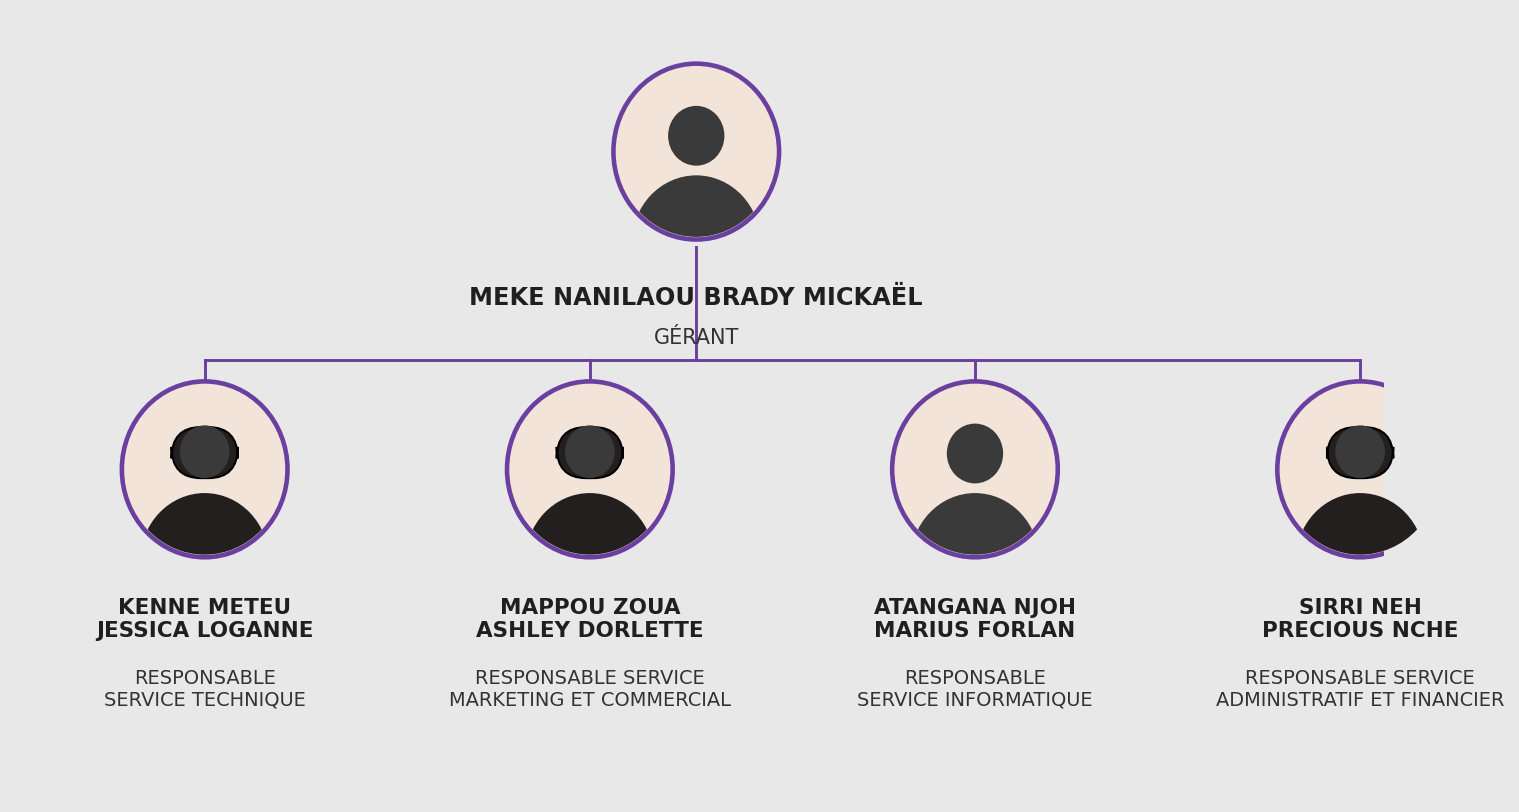
\includegraphics[width=0.9\textwidth]{capt2.png}
    \caption{Équipe managériale}
    \label{fig:equipe_manageriale}
    \tablesourcepromoteurs

\end{figure}

Le tableau ci-après présente une synthèse structurée des membres de l'équipe managériale, en mettant en lumière leurs fonctions respectives ainsi que leurs qualifications.

\begin{table}[htbp]
    \centering
    \caption{Composition de l'équipe managériale}
    \label{tab:composition_equipe}
    \renewcommand{\arraystretch}{1.5}
    \begin{tabularx}{\textwidth}{|>{\raggedright\arraybackslash}p{4cm}|>{\raggedright\arraybackslash}p{4.5cm}|X|}
        \hline
        \textbf{Postes de responsabilité} & \textbf{Responsables} & \textbf{Qualifications} \\
        \hline
        Gérant & MEKE NANILAOU BRADY MIKAEL & Ingénieur des travaux de télécommunications option Informatique et Réseau \\
        \hline
        Responsable Service Technique & KENNE METEU JESSICA LOGANNE & Ingénieur des travaux de télécommunications option Radiocommunication \\
        \hline
        Responsable Service Marketing et Commercial & MAPPOU ZOUA ASHLEY DORLETTE & Inspecteur des postes et télécommunications option Management des Télécommunications \\
        \hline
        Responsable du service informatique & ATANGANA NJOH MARIUS FORLAN & Ingénieur des travaux de télécommunications option Réseau et Télécommunications \\
        \hline
        Responsable Service Administratif et Financier & SIRRI NEH PRECIOUS NCHE & Inspecteur des postes et télécommunications option Comptabilité et Finance \\
        \hline
    \end{tabularx}
    \tablesourcepromoteurs

\end{table}

\subsubsection{Personnels à recruter}

Pour assurer le bon fonctionnement et le développement de notre système de boîte noire dédié aux conteneurs maritimes, nous allons procéder au recrutement de personnels qualifiés dont les profils, qualifications et compétences requises sont détaillés dans le tableau ci-dessous.

\begin{xltabular}{\textwidth}{|>{\raggedright\arraybackslash}p{3.4cm}|>{\centering\arraybackslash}p{0.8cm}|>{\raggedright\arraybackslash}p{3.1cm}|X|}
    \caption{Personnels à recruter} \label{tab:personnels_recruter} \\
    \hline
    \tableheadrow\thc{Poste} & \thc{Nb.} & \thc{Qualification} & \thc{Compétences} \\
    \hline
    \endfirsthead

    \multicolumn{4}{c}{\tablename~\thetable{} -- Personnels à recruter} \\
    \hline
    \tableheadrow\thc{Poste} & \thc{Nb.} & \thc{Qualification} & \thc{Compétences} \\
    \hline
    \endhead

    \endfoot
    
    \hline
    \endlastfoot

    Ingénieur en systèmes embarqués & 1 & BAC+5 en génie électronique & 
    \begin{itemize}[leftmargin=*, nosep, before=\vspace{-0.5\baselineskip}, after=\vspace{-0.5\baselineskip}]
        \item Conception et développement de systèmes d'acquisition de données embarqués
        \item Maîtrise des protocoles de communication (GPS, GPRS, satellite)
        \item Connaissance des normes maritimes (IMO, SOLAS)
        \item Intégration des capteurs (température, humidité, chocs, géolocalisation)
        \item Tests et validation des systèmes embarqués
    \end{itemize} \\
    \hline
    Ingénieur en développement logiciel & 1 & BAC+5 en informatique / Data Engineering & 
    \begin{itemize}[leftmargin=*, nosep, before=\vspace{-0.5\baselineskip}, after=\vspace{-0.5\baselineskip}]
        \item Développement d'applications de traitement et d'analyse de données
        \item Maîtrise des bases de données temps réel et des architectures cloud
        \item Développement d'interfaces de suivi et de visualisation cartographique
        \item Sécurisation des données et mise en œuvre de la cryptographie
        \item Connaissance des API de géolocalisation et de cartographie
    \end{itemize} \\
    \hline
    Responsable Technique et Qualité & 1 & BAC+3 en génie industriel / qualité & 
    \begin{itemize}[leftmargin=*, nosep, before=\vspace{-0.5\baselineskip}, after=\vspace{-0.5\baselineskip}]
        \item Assurer la conformité aux normes maritimes internationales (ISO, CE)
        \item Gestion des tests de résistance, d'étanchéité et certification (IP68, ATEX)
        \item Suivi et gestion des audits qualité et de la documentation technique
        \item Pilotage de la maintenance préventive et corrective des équipements
        \item Rédaction et mise à jour des rapports techniques et procédures qualité
    \end{itemize} \\
    \hline
    Responsable Commercial et Marketing & 1 & BAC+3 en commerce international & 
    \begin{itemize}[leftmargin=*, nosep, before=\vspace{-0.5\baselineskip}, after=\vspace{-0.5\baselineskip}]
        \item Développement et fidélisation du portefeuille clients dans le secteur
        \item Maîtrise des techniques de négociation et de vente B2B
        \item Connaissance approfondie du marché du transport maritime mondial
        \item Négociation des contrats avec les armateurs, transitaires et opérateurs
        \item Veille concurrentielle et analyse du marché
    \end{itemize} \\
    \hline
    Techniciens d'installation et de maintenance & 2 & BAC+2 en électronique / maintenance industrielle & 
    \begin{itemize}[leftmargin=*, nosep, before=\vspace{-0.5\baselineskip}, after=\vspace{-0.5\baselineskip}]
        \item Installation et configuration des boîtes noires sur les conteneurs
        \item Maintenance préventive et corrective des équipements électroniques
        \item Diagnostic et résolution des pannes matérielles et logicielles
        \item Formation et assistance technique des utilisateurs finaux
        \item Rédaction des rapports d'intervention et de suivi de maintenance
    \end{itemize} \\
    \hline
    Responsable Administratif et Juridique & 1 & BAC+3/5 en droit des affaires / administration & 
    \begin{itemize}[leftmargin=*, nosep, before=\vspace{-0.5\baselineskip}, after=\vspace{-0.5\baselineskip}]
        \item Assurer une veille juridique et réglementaire liée au secteur maritime
        \item Rédaction et suivi des contrats commerciaux, accords et conventions
        \item Gestion des contentieux et représentation de l'entreprise (justice)
        \item Capacité à planifier et organiser les tâches administratives
        \item Assurer le respect des obligations légales, fiscales et réglementaires
        \item Compétence dans la gestion de projets administratifs et institutionnels
    \end{itemize} \\
    \hline
    Secrétaire & 1 & BAC+2 en secrétariat / bureautique & 
    \begin{itemize}[leftmargin=*, nosep, before=\vspace{-0.5\baselineskip}, after=\vspace{-0.5\baselineskip}]
        \item Maîtrise des outils bureautiques (Word, Excel, PowerPoint)
        \item Rédaction et mise en forme de courriers, rapports et comptes-rendus
        \item Gestion du courrier entrant et sortant et archivage des documents
        \item Accueil physique et téléphonique des visiteurs et partenaires
        \item Organisation des réunions, agendas et déplacements professionnels
        \item Gestion administrative et suivi des dossiers du personnel
    \end{itemize} \\
    \hline
    Ménagère & 1 & BEPC / niveau primaire & 
    \begin{itemize}[leftmargin=*, nosep, before=\vspace{-0.5\baselineskip}, after=\vspace{-0.5\baselineskip}]
        \item Nettoyage et entretien quotidien des bureaux et espaces communs
        \item Lavage, repassage et entretien du linge de service
        \item Gestion et approvisionnement des produits d'entretien et ménagers
        \item Préparation et service des repas pour le personnel si nécessaire
        \item Maintien de l'hygiène et de la propreté de l'ensemble des locaux
        \item Gestion des déchets et respect des normes d'hygiène en vigueur
    \end{itemize} \\
    \hline
    Vigile & 1 & BEPC / formation en sécurité & 
    \begin{itemize}[leftmargin=*, nosep, before=\vspace{-0.5\baselineskip}, after=\vspace{-0.5\baselineskip}]
        \item Bonne condition physique et résistance à l'effort
        \item Surveillance et contrôle des accès aux locaux et installations
        \item Capacité à intervenir rapidement en cas d'incident ou d'intrusion
        \item Maîtrise des techniques de défense et de gestion des conflits
        \item Rédaction des rapports de ronde et d'incidents de sécurité
        \item Sens de la vigilance, rigueur et aptitude au travail de nuit
    \end{itemize} \\
\end{xltabular}
\noindent \textit{Source : Promoteurs 2025-2026}


\section{Étude de la faisabilité juridique et fiscale}

La présente étude vise à déterminer si et à quelles conditions le projet ARGOS est réalisable au regard des contraintes légales et fiscales applicables au Cameroun. Elle aboutit à des recommandations à mettre en œuvre, notamment en termes contractuel et fiscal, et constitue une étape primordiale afin de ne pas s'engager dans un projet qui pourrait se révéler illégal après avoir consenti des investissements importants.


\subsection{Faisabilité juridique}

Afin de préserver la force probante des données et de garantir la conformité réglementaire de la solution, plusieurs risques juridiques critiques doivent être anticipés dès la phase de conception a savoir :
\begin{itemize}
    \item \textbf{Preuve légale des données :} en cas de litige, la valeur probante des données dépend notamment de la capacité à démontrer leur intégrité, leur traçabilité et les conditions de leur conservation. Une évaluation technique indépendante du dispositif et de la chaîne de données peut renforcer cette démonstration, sans constituer à elle seule une garantie automatique d'admission de la preuve.
    \item \textbf{Conformité maritime :} l'emploi du dispositif doit être examiné au regard des règles applicables au conteneur et à la cargaison, notamment la convention SOLAS et, en présence de marchandises dangereuses, le code IMDG\cite{imo_solas,imo_imdg}. L'OMI édicte ces instruments internationaux, mais n'homologue pas directement chaque boîtier commercialisé. Les essais, homologations et certificats requis doivent être obtenus auprès des autorités nationales compétentes et, selon le cas, d'organismes techniques reconnus.
    \item \textbf{Protection des données et RGPD :} le RGPD s'applique lorsque le traitement entre dans son champ territorial et porte sur des données relatives à une personne physique identifiée ou identifiable, notamment des données de localisation. Le simple transit d'un conteneur dans l'Union européenne ne suffit donc pas, à lui seul, à déclencher l'application du règlement\cite{rgpd_officiel}.
    \item \textbf{Télécommunications et importation :} les équipements de communications électroniques ou installations radioélectriques doivent faire l'objet des formalités d'homologation applicables auprès de l'Agence de Régulation des Télécommunications (ART). Le dossier comprend notamment les spécifications techniques, la déclaration de conformité du fabricant et les rapports d'essais\cite{art_homologation}. Le classement tarifaire et les droits de douane doivent être confirmés auprès de la Direction Générale des Douanes avant l'importation ; aucun taux forfaitaire de 40~\% n'est retenu ici faute de source officielle vérifiée.
\end{itemize}

La maîtrise de ces quatre enjeux juridiques des valeur probante des données, des conformité maritime internationale, des protection des données personnelles et régularité douanière et conditionne la solidité juridique du projet Argos et confirme sa faisabilité sur ce plan, sous réserve des démarches de certification et d'homologation évoquées.

\subsubsection{Statut juridique}

La forme de statut juridique (ou forme juridique) d'une entreprise désigne le cadre légal imposé à une activité économique. L'article 4 de l'Acte uniforme OHADA relatif au droit des sociétés commerciales et du groupement d'intérêt économique dispose :

« la société commerciale est créée par deux ou plusieurs personnes qui conviennent par contrat, d'affecter à une activité, des biens en numéraire ou en nature, dans le but de partager les bénéfices ou de profiter de l'économie qui pourra en résulter »\cite{ohada_auscgie}.

Les règles applicables régissant l'activité de l'entreprise sont donc tributaires de ce statut. Le choix du statut entraîne diverses conséquences notamment juridiques au sein d'une entreprise.

Dans le cadre de notre projet ARGOS, nous optons pour le statut de Société à Responsabilité Limitée (SARL) pour les raisons suivantes :

\begin{table}[htbp]
    \centering
    \caption{Justification du choix de la SARL}
    \label{tab:choix_sarl}
    \renewcommand{\arraystretch}{1.5}
    \begin{tabularx}{\textwidth}{|>{\raggedright\arraybackslash}p{4cm}|X|}
        \hline
        \textbf{Critère} & \textbf{Justification} \\
        \hline
        Limitation des risques & La responsibilite des associés est limitée à leurs apports, protégeant ainsi le patrimoine personnel des promoteurs. \\
        \hline
        Protection sociale & Affiliation à la CNPS des travailleurs salariés employés par la société, dans les conditions prévues par la réglementation sociale. \\
        \hline
        Accès au code des investissements & Possibilité de bénéficier des mesures incitatives prévues par la réglementation camerounaise. \\
        \hline
        Capital social & Capital fixé par les associés dans le respect des dispositions OHADA et nationales applicables. \\
        \hline
        Protection patrimoniale & Protection du patrimoine personnel en cas de faillite. \\
        \hline
        Crédibilité & Recherche d'une crédibilité auprès des investisseurs et partenaires institutionnels. \\
        \hline
    \end{tabularx}
    \tablesourcepromoteurs
\end{table}
La fiche d'identité de l'entreprise se présente comme suit :
\begin{table}[htbp]
    \centering
    \caption{Fiche d'identité de l'entreprise ARGOS}
    \label{tab:fiche_identite}
    \renewcommand{\arraystretch}{1.5}
    \begin{tabularx}{\textwidth}{|>{\raggedright\arraybackslash}p{4cm}|X|}
        \hline
        \textbf{Élément} & \textbf{Information} \\
        \hline
        Raison sociale & ARGOS SARL \\
        \hline
        Forme juridique & SARL \\
        \hline
        Capital & 20 000 000 FCFA \\
        \hline
        Activité & Conception, fabrication et commercialisation de solutions de traçabilité et de monitoring intelligent pour conteneurs maritimes \\
        \hline
        Secteur d'activité & Télécommunications, TIC, Électronique, IoT (Internet des Objets) \\
        \hline
        Produits & Dispositif embarqué « boîte noire » ARGOS + Plateforme de supervision logicielle \\
        \hline
        Siège social & Douala (zone portuaire stratégique) \\
        \hline
        Téléphone & 220 10 29 07 \\
        \hline
        E-mail & Argos@argos-sarl.com \\
        \hline
        Année de création & 2026 \\
        \hline
    \end{tabularx}
    \tablesourcepromoteurs
\end{table}

L’analyse comparative des statuts juridiques conduit à l'adoption de la Société à Responsabilité Limitée (SARL), dont les motivations stratégiques sont synthétisées dans le Tableau \ref{tab:choix_sarl}. Ce tableau met en lumière les avantages majeurs de cette forme juridique, notamment la limitation de la responsabilité des associés à leurs apports et protégeant ainsi leur patrimoine personnel, leur accès aux avantages du Code des investissements au Cameroun, ainsi qu'une crédibilité renforcée auprès des partenaires financiers et institutionnels.

Dans la continuité de ce choix organisationnel, la formalisation de l'entreprise se concrétise à travers sa carte d'identité officielle présentée dans le Tableau \ref{tab:fiche_identite}. Ce récapitulatif structure l'ensemble des informations clés d'ARGOS SARL et de sa raison sociale à son capital social fixé à 20\,000\,000 FCFA, en passant par son positionnement au cœur du pôle stratégique de Douala et ses domaines d'expertise en IoT et télécommunications. Ce tableau constitue ainsi la boussole institutionnelle de l'entreprise, garantissant sa lisibilité auprès des autorités réglementaires et des acteurs de la chaîne logistique.

\subsubsection{Régime d'imposition de l'entreprise}

Le régime d'imposition est un dispositif fiscal qui fixe l'ensemble des règles facilitant la détermination des impôts et des taxes. Conformément aux dispositions de l'article 93 du Code Général des Impôts (CGI), les contribuables relèvent des régimes ci-après, déterminés notamment en fonction du chiffre d'affaires réalisé\cite{cgi_cameroun}.

\begin{table}[htbp]
    \centering
    \caption{Régimes d'imposition au Cameroun}
    \label{tab:regimes_imposition}
    \renewcommand{\arraystretch}{1.5}
    \begin{tabularx}{\textwidth}{|>{\raggedright\arraybackslash}p{4cm}|>{\raggedright\arraybackslash}p{5cm}|X|}
        \hline
        \textbf{Régime} & \textbf{Conditions} & \textbf{Caractéristiques} \\
        \hline
        Régime de l'impôt libératoire & CA annuel HT $<$ 10 000 000 FCFA & Entreprises individuelles uniquement \\
        \hline
        Régime simplifié & CA annuel HT $\geq$ 10 000 000 FCFA et $<$ 50 000 000 FCFA & Entreprises individuelles et personnes morales \\
        \hline
        Régime du réel & CA annuel HT $\geq$ 50 000 000 FCFA & Entreprises individuelles et personnes morales \\
        \hline
    \end{tabularx}
    \tablesourcepromoteurs

\end{table}

\paragraph{Régime applicable à ARGOS :}
Au vu de notre chiffre d'affaires prévisionnel (186 685 000 FCFA la première année, 465 500 000 FCFA la deuxième année, 928 300 000 FCFA la troisième année), notre entreprise relèvera du régime réel dès la première année d'activité\cite{cgi_cameroun}.

\paragraph{L'impôt sur les sociétés (IS) applicable aux SARL :}
Les SARL entrent dans le champ de l'impôt sur les sociétés. Le CGI fixe le taux de droit commun à 30~\% et prévoit un taux de 25~\% pour les contribuables dont le chiffre d'affaires est inférieur ou égal à 3 milliards de FCFA, sous réserve des autres conditions et régimes particuliers prévus par les textes\cite{cgi_cameroun}.

\paragraph{Exonérations fiscales pour les nouvelles entreprises (Loi de Finances 2025) :}
La fiscalité camerounaise prévoit des mesures incitatives, mais celles-ci ne sont pas automatiques du seul fait de la création d'une société ou de son activité dans les TIC. Leur bénéfice dépend de l'éligibilité du projet, de l'obtention de l'agrément requis et du respect des obligations prévues par le régime applicable\cite{incitations2025}.

ARGOS devra donc vérifier son éligibilité avant d'inscrire un avantage fiscal dans ses prévisions. Les avantages susceptibles d'être sollicités peuvent porter sur :
\begin{itemize}
    \item les mesures prévues par le régime d'incitation à l'investissement auquel le projet serait agréé ;
    \item les facilités fiscales ou douanières expressément mentionnées dans la décision d'agrément ;
    \item les dispositifs sectoriels auxquels l'entreprise démontrerait son éligibilité.
\end{itemize}
\textbf{Attention :} Les exonérations sont conditionnées au respect des obligations déclaratives et comptables. En cas de non-respect, l'administration fiscale peut retirer l'avantage et appliquer l'IS rétroactivement.

\subsubsection{Obligations de l'entreprise}

Les obligations sociales de notre entreprise ARGOS sont nombreuses. Nous les présentons ci-après.
\begin{table}[htbp]
    \centering
    \caption{Obligations fiscales de l'entreprise}
    \label{tab:obligations_fiscales}
    \renewcommand{\arraystretch}{1.5}
    \begin{tabularx}{\textwidth}{|>{\raggedright\arraybackslash}p{4cm}|X|p{3cm}|}
        \hline
        \textbf{Obligation} & \textbf{Description} & \textbf{Échéance} \\
        \hline
        Numéro de contribuable & Acquisition obligatoire avant le début de l'activité & Immédiat \\
        \hline
        IRPP & Déclaration et paiement des retenues sur salaires & Mensuel \\
        \hline
        Immatriculation fiscale & Obtention de l'attestation d'immatriculation fiscale & À la création \\
        \hline
        Enregistrement du bail & 10~\% du montant global du loyer annuel si l'entreprise est locataire & À la signature \\
        \hline
        Précompte sur loyer & Retenue de 5~\% sur le loyer & Mensuel \\
        \hline
        Taxe sur la publicité & Plaques publicitaires site commerciale. & Annuel \\
        \hline
        TVA & Déclaration et paiement (taux : 19,25~\%) & Mensuel/Trimestriel \\
        \hline
        Patente & Déclaration et paiement, sauf exonération expressément applicable & Annuel \\
        \hline
        Acompte sur IS & 1,5~\% + CAC sur l'IS & Mensuel \\
        \hline
        IS de clôture & Complément d'impôt sur les sociétés en fin d'exercice & Annuel \\
        \hline
    \end{tabularx}
    \noindent\textit{Source : Promoteurs, à partir du Code général des impôts\cite{cgi_cameroun}.}
\end{table}

\noindent Le Tableau~\ref{tab:obligations_fiscales} dresse un panorama exhaustif du cadre fiscal régissant les activités d'ARGOS SARL au Cameroun. L'importance de ce tableau réside dans sa capacité à cartographier rigoureusement les différentes échéances (mensuelles, annuelles ou ponctuelles) et les taxes applicables (TVA, IRPP, acomptes sur IS). Cette visibilité fiscale est indispensable pour l'entreprise afin d'anticiper sa trésorerie, de planifier ses charges d'exploitation et de garantir une conformité totale avec l'administration fiscale, sécurisant ainsi la pérennité financière de la structure.

\bigskip

\begin{table}[htbp]
    \centering
    \caption{Obligations sociales de l'entreprise}
    \label{tab:obligations_sociales}
    \renewcommand{\arraystretch}{1.5}
    \begin{tabularx}{\textwidth}{|>{\raggedright\arraybackslash}p{4cm}|X|}
        \hline
        \textbf{Obligation} & \textbf{Description} \\
        \hline
        Immatriculation du personnel & Déclaration à la CNPS de tout personnel employé \\
        \hline
        Cotisations CNPS & Déclaration et paiement des retenues sur salaire (allocations familiales, pension vieillesse, accidents de travail) \\
        \hline
        DIPE & Tenue du Document d'Information sur le Personnel Employé \\
        \hline
        Registres obligatoires & Tenue du livret de paie, du registre du personnel, du règlement intérieur, des fascicules 1, 2 et 3 du personnel employé \\
        \hline
    \end{tabularx}
    \noindent\textit{Source : CNPS et Code général des impôts\cite{cnps_employeurs,cgi_cameroun}.}
\end{table}

\noindent le Tableau~\ref{tab:obligations_sociales} synthétise les exigences réglementaires en matière de gestion des ressources humaines et de protection sociale. Ce récapitulatif met en lumière l'engagement de l'entreprise envers ses collaborateurs à travers l'immatriculation auprès de la CNPS, la gestion rigoureuse des cotisations et la tenue des documents obligatoires (DIPE, registres de paie). L'importance de ce dispositif réside dans le respect des droits des salariés, la prévention des risques de contentieux avec les institutions de contrôle du travail et la construction d'un climat social stable et professionnel au sein d'ARGOS SARL.

\paragraph{Obligations liées à la protection des données personnelles (Loi n°2024/017) :}
La loi n°2024/017 du 23 décembre 2024 encadre au Cameroun la collecte et les autres opérations de traitement portant sur des données à caractère personnel. Les traitements mis en œuvre par ARGOS doivent être examinés et mis en conformité avec ce texte\cite{loi2024_donnees}.
Notre plateforme ARGOS étant amenée à traiter des données de géolocalisation et des informations sensibles sur les marchandises et les conteneurs, nous devons Obtenir le consentement explicite des utilisateurs pour la collecte et le traitement des données , Assurer la transparence sur les finalités du traitement , Garantir les droits des personnes (accès, rectification, effacement, opposition, portabilité) ,Notifier toute violation de données à l'autorité compétente ,Encadrer les transferts internationaux de données.

\textbf{Sanctions :} le non-respect de la loi expose le responsable du traitement aux sanctions administratives et pénales prévues par ce texte\cite{loi2024_donnees}.

\subsubsection{Processus de création de l'entreprise}

La formalisation d'une société s'effectue auprès du Centre de Formalités de Création d'Entreprises (CFCE), qui centralise les principales démarches de création. Le dossier d'une société commerciale comprend notamment les statuts, la déclaration requise pour la SARL, la liste des dirigeants ou associés et un plan de localisation\cite{minpmeesa_cfce}.

\paragraph{Phase 1 : Création de l'entreprise au CFCE }

\indent Pour une SARL, la procédure comprend notamment les opérations suivantes :
\begin{itemize}
    \item établissement des statuts dans la forme requise et préparation des déclarations de constitution ;
    \item dépôt du dossier au CFCE pour l'immatriculation au RCCM, l'immatriculation fiscale et les formalités sociales applicables.
\end{itemize}

\paragraph{Phase 2 : Enregistrement de l'entreprise}

\indent Les documents nécessaires pour l'enregistrement auprès du centre des impôts sont :
\begin{itemize}
    \item Le Registre du commerce ;
    \item Les statuts ;
    \item L'attestation d'immatriculation ;
    \item Le plan de localisation ;
    \item Le contrat de bail.
\end{itemize}

\subsubsection{Bilan du coût total de création d'entreprise}

La création légale de la société ARGOS SARL implique un ensemble de démarches administratives, notariales et fiscales. Afin de budgétiser précisément la phase de lancement, le tableau ci-dessous récapitule l'intégralité des frais liés à l'immatriculation et à l'obtention des documents officiels. Ce bilan financier constitue le coût d'entrée indispensable pour formaliser l'existence juridique de l'entreprise.

\begin{table}[H]
    \centering
    \caption{Coût de création de l'entreprise}
    \label{tab:cout_creation}
    \renewcommand{\arraystretch}{1.5}
    \begin{tabularx}{\textwidth}{|>{\raggedright\arraybackslash}p{3.5cm}|>{\raggedright\arraybackslash}p{4cm}|c|X|}
        \hline
        \textbf{Organe concerné} & \textbf{Pièces à obtenir} & \textbf{Montant (FCFA)} & \textbf{Observation} \\
        \hline
        Greffe du tribunal de 1ère instance & Extrait du casier judiciaire & 12 500 & 2 500 FCFA $\times$ 5 associés \\
        \hline
        CNPS & Attestation de soumission CNPS & 8 000 & 6 000 FCFA + 2 timbres de 1 000 FCFA \\
        \hline
        CNPS & Attestation de non-utilisation du personnel salarié & 2 500 & \\
        \hline
        Centre des impôts & Carte de contribuable & Exonéré & Exonération pendant les 5 premières années \\
        \hline
        Centre des impôts & Attestation d'exonération à la patente & Exonéré & Exonération pendant les 5 premières années \\
        \hline
        RCCM & Attestation d'immatriculation & 41 500 minimum & Montant minimal publié par le MINPMEESA ; coût variable selon le dossier \\
        \hline
        Notaire & Frais notariés & 80 000 & Mise en place de la SARL \\
        \hline
        \textbf{Total estimatif} & \multicolumn{3}{l|}{\textbf{144 500 FCFA minimum, à confirmer par devis et quittances}} \\
        \hline
    \end{tabularx}
    \noindent\textit{Source : estimations des promoteurs ; montant minimal du RCCM vérifié auprès du MINPMEESA\cite{minpmeesa_cfce}.}
\end{table}

\subsubsection{Bilan des risques et opportunités}

Le déploiement d'une solution technologique innovante dans le secteur maritime expose naturellement l'entreprise à divers aléas. Pour garantir la viabilité du projet ARGOS, il est crucial de cartographier ces menaces potentielles. Le tableau suivant identifie et catégorise les principaux risques juridiques, fiscaux et sectoriels susceptibles d'impacter nos opérations.

\begin{table}[H]
    \centering
    \caption{Identification des risques}
    \label{tab:identification_risques}
    \renewcommand{\arraystretch}{1.5}
    \begin{tabularx}{\textwidth}{|>{\raggedright\arraybackslash}p{4cm}|X|}
        \hline
        \textbf{Catégorie} & \textbf{Description des risques} \\
        \hline
        Risques juridiques & Non-conformité à la loi 2024/017 sur la protection des données personnelles; Contentieux liés à la responsabilité des données de localisation; Évolution des réglementations maritimes (OMI). \\
        \hline
        Risques fiscaux & Perte des avantages fiscaux en cas de non-respect des obligations déclaratives; Requalification fiscale du régime d'imposition; Changement de la législation fiscale. \\
        \hline
        Risques sectoriels & Concurrence des multinationales; Évolution rapide des technologies; Dépendance aux fournisseurs de composants électroniques. \\
        \hline
    \end{tabularx}
    \tablesourcepromoteurs
\end{table}

L'identification de ces vulnérabilités n'est qu'une première étape ; elle doit impérativement s'accompagner de mesures préventives et correctives. Ainsi, le tableau ci-après détaille la stratégie de gestion des risques adoptée par ARGOS pour atténuer ces menaces, sécuriser l'investissement et transformer ces défis en avantages concurrentiels.

\begin{table}[H]
    \centering
    \caption{Plan d'action contre les risques}
    \label{tab:plan_action_risques}
    \renewcommand{\arraystretch}{1.5}
    \begin{tabularx}{\textwidth}{|>{\raggedright\arraybackslash}p{4cm}|X|}
        \hline
        \textbf{Risque} & \textbf{Plan d'action} \\
        \hline
        Risques juridiques & Désigner un Délégué à la Protection des Données (DPO); Mettre en conformité la plateforme avant le 23 juin 2026; Rédiger des conditions générales d'utilisation et une politique de confidentialité claires. \\
        \hline
        Risques fiscaux & Se faire accompagner par un expert-comptable; Respecter scrupuleusement les délais de déclaration; Conserver toutes les preuves d'éligibilité aux exonérations. \\
        \hline
        Risques sectoriels & Placer l'innovation au cœur de la stratégie; Diversifier les fournisseurs; Surveiller l'évolution de la concurrence et du marché. \\
        \hline
    \end{tabularx}
    \tablesourcepromoteurs
\end{table}


\subsection{Étude de la faisabilité fiscale}

Sur le plan fiscal, plusieurs démarches conditionnent la viabilité du projet ARGOS et doivent être anticipées afin d'éviter tout blocage administratif ou surcoût imprévu, lesquelles s'articulent autour des points suivants :
\begin{itemize}
    \item \textbf{Agrément aux incitations à l'investissement :} ARGOS peut déposer une demande auprès du guichet compétent prévu par le régime des incitations à l'investissement. La nature et la durée des avantages ne doivent être intégrées au plan financier qu'après vérification de l'éligibilité et délivrance d'un agrément précisant les facilités accordées\cite{incitations2025}.
    \item \textbf{Classement tarifaire douanier :} il est nécessaire de démontrer auprès de la Direction Générale des Douanes (DGD) que le boîtier Argos ne relève pas de la catégorie générique des « appareils électroniques », dont le taux de taxation est plus élevé, mais d'une catégorie plus adaptée à sa fonction de dispositif de traçabilité logistique, afin d'obtenir un classement tarifaire plus favorable.
    \item \textbf{Autorisations techniques et coordination portuaire :} une coordination avec le Port Autonome de Douala peut faciliter l'expérimentation en zone portuaire, mais elle ne supprime pas automatiquement les taxes ou redevances applicables. L'homologation d'un équipement de communications électroniques ou radioélectrique relève de la procédure publiée par l'ART\cite{art_homologation}.
\end{itemize}

La sécurisation de ces trois démarches fiscales et douanières conditionne la rentabilité du modèle économique d'Argos et confirme la faisabilité fiscale du projet, sous réserve de leur mise en œuvre effective.


\subsubsection{Synthèse}

L'étude de faisabilité juridique et fiscale du projet ARGOS démontre que la création d'une SARL est juridiquement viable et fiscalement avantageuse dans le contexte camerounais actuel.

\begin{table}[htbp]
    \centering
    \caption{Synthèse de l'étude juridique et fiscale}
    \label{tab:synthese_etude}
    \renewcommand{\arraystretch}{1.5}
    \begin{tabularx}{\textwidth}{|>{\raggedright\arraybackslash}p{4cm}|X|}
        \hline
        \textbf{Aspect} & \textbf{Constat} \\
        \hline
        Statut juridique & SARL adaptée pour limiter les risques et bénéficier d'une crédibilité auprès des investisseurs. \\
        \hline
        Régime fiscal & Régime réel dès la première année au regard du chiffre d'affaires prévisionnel ; avantages fiscaux uniquement sous réserve d'éligibilité et d'agrément. \\
        \hline
        Protection des données & Obligation de conformité des traitements à la loi n°2024/017. \\
        \hline
        Coût de création & Environ 124 500 FCFA (hors capital social). \\
        \hline
        Capital social & 20 000 000 FCFA (apports des 5 associés fondateurs). \\
        \hline
    \end{tabularx}
    \tablesourcepromoteurs
\end{table}

 ce chapitre a permis de démontrer la faisabilité globale du projet ARGOS en validant successivement ses dimensions technique, organisationnelle, juridique et fiscale. Sur le plan technique, les solutions apportées pour surmonter les défis critiques — tels que l'autonomie énergétique en haute mer, la connectivité en zone blanche, la sécurité physique du boîtier et la cybersécurité des données confirment la robustesse de l'architecture retenue. L'analyse organisationnelle a mis en évidence une structure managériale solide (SARL) portée par une équipe aux compétences complémentaires, soutenue par un plan de recrutement ciblé pour accompagner la croissance de l'entreprise. Enfin, l'étude juridique et fiscale a validé le choix de la Société à Responsabilité Limitée (SARL), garantissant une protection patrimoniale adéquate, une conformité stricte aux réglementations en vigueur (notamment la loi n°2024/017 sur la protection des données) et un accès stratégique aux mesures incitatives du code des investissements camerounais. Ces fondations étant posées et sécurisées, il convient à présent d'évaluer la rentabilité et la robustesse économique de ce modèle à travers l'étude de viabilité financière, objet du chapitre suivant.
